\subsection{Gestion de version}\label{subsec:gestion-de-version}

La gestion de version est une pratique essentielle dans tout projet de développement logiciel.
Dans le cadre de ce projet, nous avons utilisé Git comme système de gestion de versions et GitHub comme hébergement pour notre code source.

Au début du projet, j'ai opté pour l'utilisation d'une seule branche durant la majeure partie de la première phase.
Cette stratégie était adéquate pour répondre aux besoins initiaux du projet, en maintenant une simplicité de gestion.

Toutefois, avec la publication du projet sur DockerHub et l'instauration de l'intégration et du déploiement continus (CI/CD), il est devenu clair que l'utilisation d'une seule branche n'était plus la meilleure option.
J'ai alors introduit une branche de développement distincte, permettant d'expérimenter et d'innover sans perturber la version en production.

Pour la rédaction de ce rapport, j'ai également créé une branche spécifique, ce qui a permis de travailler sur la documentation sans interférer avec le code de l'application.

La gestion de l'infrastructure du projet a été organisée dans un second dépôt GitHub.
Cette décision a été motivée par le fait que l'infrastructure du projet s'inspirait d'un autre projet existant que j'ai forké.
Avoir un dépôt distinct pour l'infrastructure a permis de maintenir une séparation claire entre le code de l'application et la gestion de l'infrastructure.

\subsection{Intégration et déploiement continu (CI/CD)}\label{subsec:integration-et-deploiement-continu-(ci/cd)}

L'intégration continue (CI) a été mise en œuvre grâce à des tests automatisés sur une grande partie des composants du back-end et du front-end.

\begin{figure}[H]
    \begin{minipage}[b]{0.5\textwidth}
        \centering
        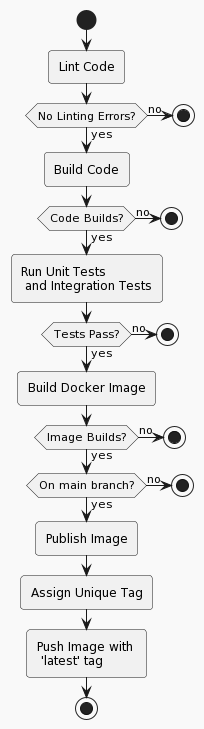
\includegraphics[height=0.3\textheight, keepaspectratio]{images/ci_workflow}
        \caption{Workflow d'intégration continue}
        \label{fig:ci_workflow}
    \end{minipage}%
    \begin{minipage}[b]{0.5\textwidth}
        Le workflow de CI est le suivant :

        \begin{itemize}
            \item Lint du code : vérification des erreurs de syntaxe.
            \item Build du code : si aucune erreur de linting n'est détectée, je peux construire le code.
            \item Tests unitaires et d'intégration : si le code se construit correctement, je lance les tests.
            \item Construction de l'image Docker : si les tests passent, je construis l'image du conteneur.
            \item Publication de l'image : si la construction de l'image réussit, je la publie sur DockerHub (seulement si je suis sur la branche principale).
        \end{itemize}
    \end{minipage}
\end{figure}

En ce qui concerne le déploiement continu (CD), j'utilise un conteneur Watchtower qui, via le socket Docker, vérifie régulièrement si la version du conteneur utilisée correspond bien à celle souhaitée.
Watchtower vérifie également la signature du conteneur en plus de son tag, ce qui lui permet de mettre à jour un conteneur avec le tag "latest" lorsque l'image change.
Watchtower compare régulièrement la version courante des conteneurs à celle hébergée sur DockerHub et si elles ne correspondent pas, alors le conteneur est mis à jour.

\subsubsection{Tests de l'API}
L'API est testée à travers plusieurs types de tests, principalement des tests unitaires qui se concentrent sur une fonction
spécifique de manière isolée et des tests d'intégration qui testent l'API de bout en bout.\\

Les tests d'intégration, bien qu'étant plus complexes à mettre en œuvre, ont été particulièrement intéressants.
Pour faciliter leur mise en place, j'ai créé un gestionnaire de tests qui, en plus des fonctions de mock, me permet de préparer l'application dans un état connu.
Par exemple, si le test consiste à vérifier que les événements sont accessibles via l'API, le gestionnaire de tests me permet de configurer des utilisateurs, des adresses, des pays et des événements.
Grâce à ce gestionnaire de tests, je peux ajouter des tests dans différents états du serveur.

\subsubsection{Tests de l'interface web}
Pour tester l'interface web, j'utilise Karma et Jasmine.
Ces outils me permettent de tester le comportement directement dans le navigateur, et donc de vérifier que les différents composants fonctionnent comme prévu.
Grâce à ces outils, je peux tester l'interface utilisateur de manière directe et fiable.

\subsection{Conclusion}\label{subsec:conclusion}

La gestion de version a été un aspect crucial de ce projet.
L'adoption d'une approche adaptative, passant d'une seule branche à plusieurs branches en fonction des besoins du projet, a prouvé son efficacité.
De même, l'implémentation des pratiques de CI/CD a grandement amélioré le flux de travail et la qualité de l'application, rendant le processus de développement plus fluide et fiable.